\DocumentMetadata{
	lang		= eng-US,
	pdfstandard	= A-3u,
	pdfversion	= 1.7,
}

\documentclass[colorlinks,upint,balance]{asmeconf}

\usepackage{graphicx}

\hypersetup{%
	pdfauthor={J.C. Vaught},
	pdftitle={Comparison of Gain Management Strategies for Target Resolution on Low-Bit Marine Radar},
	pdfkeywords={marine radar, gain sweep, dynamic range, X-Band, HDR, target resolution},
}

\begin{document}

\ConfName{Proceedings of the ASME 2026\linebreak International Design Engineering Technical Conferences \&\linebreak Computers and Information in Engineering Conference}
\ConfAcronym{IDETC/CIE 2026}
\ConfDate{August 23--26, 2026}
\ConfCity{Houston, TX}
\PaperNo{IDETC2026-XXXXX}

\title{Comparison of Gain Management Strategies for Target Resolution on Low-Bit Marine Radar}

\SetAuthors{%
	J.C. Vaught\affil{1}\CorrespondingAuthor{jvaught@sc.edu},
	Douglas Cahl\affil{1},
	Yi Wang\affil{1}
}

\SetAffiliation{1}{Department of Mechanical Engineering, University of South Carolina, Columbia, SC}

\maketitle

\keywords{marine radar, gain sweep, dynamic range extension, X-Band, target resolution, HDR}

% ====================================================================
% ABSTRACT
% ====================================================================
\begin{abstract}
Commodity X-Band marine radars digitize returns at low bit depths, typically four bits, imposing a fundamental tradeoff between receiver sensitivity and target resolution. At high gain, weak targets become visible but strong reflectors saturate and merge. At low gain, individual strong targets are well-resolved but weaker objects disappear entirely. This paper presents and compares three strategies for managing this tradeoff on a 4-bit intensity-only X-Band radar interfaced with a programmable gain controller. The first strategy sweeps receiver gain across its full range to reconstruct high-dynamic-range reflectivity profiles of stationary targets, analogous to exposure bracketing in computational photography. The second strategy sweeps both gain and pulse width for richer characterization at the cost of reduced rotation rate. The third strategy forgoes parameter sweeping entirely, operating at fixed high gain and exploiting temporal signal intermittency to resolve merged targets. Experimental results collected against metal navigation buoys and land features demonstrate the conditions under which each approach is preferable. The gain-sweep method achieves effective dynamic range well beyond the native 4-bit resolution at full rotation speed, while temporal filtering provides comparable discrimination for targets exhibiting intermittent returns without introducing motion artifacts in dynamic scenes.
\end{abstract}


% ====================================================================
% 1  INTRODUCTION
% ====================================================================
\section{Introduction}

X-Band marine radar has been the cornerstone of maritime situational awareness for over half a century, providing all-weather, day-and-night obstacle detection that no optical sensor can match~\cite{Skolnik2001Radar}. As autonomous surface vessels (ASVs) move from research prototypes toward operational deployment, radar has become pivotal to their perception stacks~\cite{Han2020ARAGON, Chung2023Pohang}. However, a fundamental limitation has persisted across decades of radar development: commodity marine radars digitize echo returns at extremely low bit depths. A 4-bit analog-to-digital converter produces only 16 discrete intensity levels per range cell, compressing the vast diversity of target reflectivities in a waterway scene into a handful of quantization bins~\cite{Skolnik2001Radar, Richards2014Fundamentals}.

This constraint forces a brutal tradeoff. At high receiver gain, weak targets such as navigation buoys and channel markers emerge from the noise floor, but strong reflectors---nearby land, bridge abutments, large vessels---saturate the digitizer and merge into featureless blobs. At low gain, strong targets remain individually resolved, but objects of critical navigational interest vanish entirely~\cite{Ward2013Marine}. Cho et al.~\cite{Cho2025AdaptiveSTC} demonstrated this problem directly in the context of uncrewed surface vehicles, showing that adjusting gain to suppress sea clutter simultaneously eliminated desired targets from the radar display. No single fixed gain setting can satisfy both demands.

The radar community has long sought to resolve this tension. Sensitivity time control (STC), which attenuates near-range returns with a $1/R^4$ gain curve, was among the earliest countermeasures~\cite{Watts2016STC}. While effective at reducing range-dependent clutter, STC operates purely as a function of range and cannot distinguish between clutter and targets at the same distance---setting STC aggressively enough to suppress sea clutter can simultaneously eliminate small close-range targets. Constant false alarm rate (CFAR) processing, pioneered by Rohling~\cite{Rohling1983CFAR} at the Technical University of Hamburg-Harburg, adapts detection thresholds to local clutter statistics and remains widely deployed. Yet CFAR operates on single-scan data and does not extend the digitizer's bit depth; it determines \textit{whether} a target exists, but cannot recover \textit{how strong} it is beyond the 16 available levels. Wen et al.~\cite{Wen2022SpatioTemporal} at Harbin Engineering University extended CFAR into the spatio-temporal domain using 3D-FFT filtering across marine radar image sequences, achieving up to 15.3~dB of signal-to-noise improvement---but their method, too, operates within the quantization limits of each individual frame.

More recently, deep learning methods have been brought to bear on the problem. Baird et al.~\cite{Baird2020CNNLSTM} at Carleton University and Defence Research and Development Canada combined convolutional and recurrent architectures to augment target detection on real maritime surveillance radar data. Chen et al.~\cite{Chen2021PPInet} at Xidian University achieved 15\% detection improvement over CA-CFAR using a YOLOv3-based network operating directly on radar PPI imagery. Wang and Li~\cite{Wang2023SALALSTM} at the Chinese Academy of Sciences introduced self-adaptive LSTM architectures that learn to distinguish targets from sea clutter in pulse-compressed radar echo sequences. These methods have demonstrated impressive detection performance on standard radar imagery. However, they share a fundamental limitation: a neural network trained on 4-bit data can learn to detect targets with high accuracy, but it cannot recover radiometric information that the digitizer never captured. The dynamic range ceiling is set by the hardware, and no amount of post-processing can break through it.

\begin{figure*}[t]
\centering
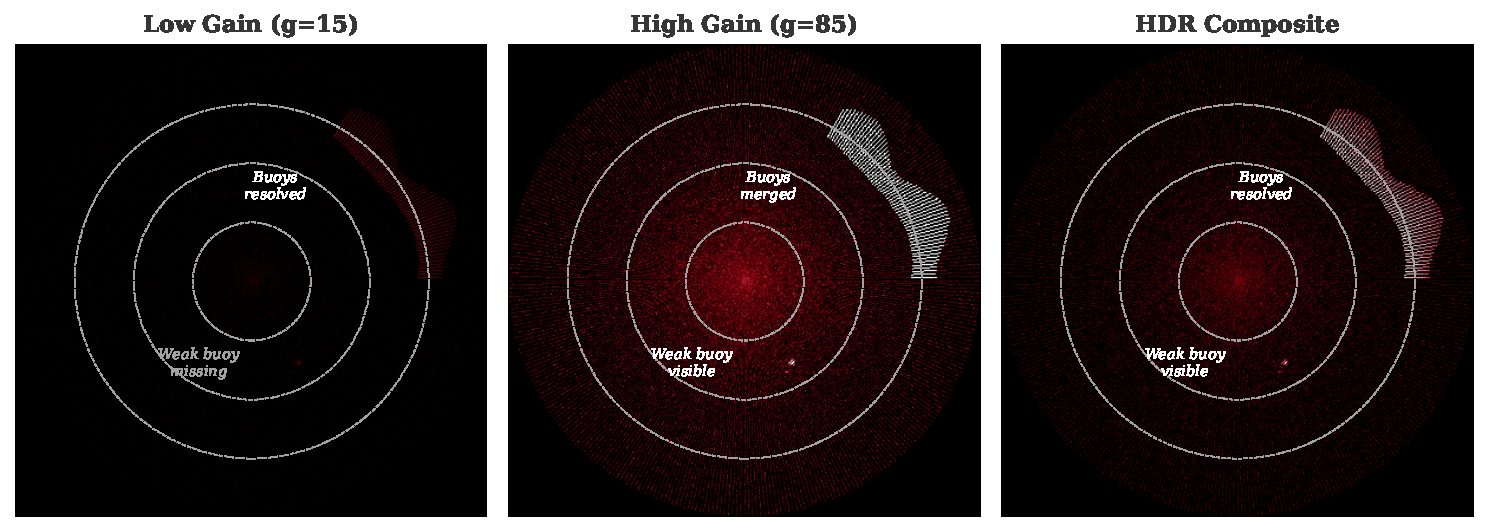
\includegraphics[width=\textwidth]{figures/fig1_gain_tradeoff.pdf}
\caption{The gain tradeoff on a 4-bit marine radar. Left: at low gain, strong targets are individually resolved but weak targets are invisible. Center: at high gain, weak targets appear but strong reflectors saturate and merge. Right: HDR composite from a full gain sweep recovers both target separation and weak target detection. \textit{Placeholder---replace with real radar data.}}
\label{fig:gain_tradeoff}
\end{figure*}

Meanwhile, the computational photography community solved an analogous problem decades ago. Debevec and Malik~\cite{Debevec1997HDR} at UC~Berkeley demonstrated in 1997 that multiple photographs taken at different exposure settings could be fused to recover a high dynamic range (HDR) radiance map far exceeding the bit depth of any single image. Mann and Picard~\cite{Mann1995HDR} at MIT had introduced exposure bracketing for dynamic range extension two years earlier. Mertens et al.~\cite{Mertens2009ExposureFusion} at Hasselt University later showed that exposure fusion could be performed without explicit HDR conversion, and Hasinoff et al.~\cite{Hasinoff2010NoiseOptimal} at MIT optimized the capture schedule itself, demonstrating that not all exposures need equal weight. These techniques are now ubiquitous in consumer cameras. Arnold~\cite{Arnold2025HDRSonarRadar} recently applied HDR rendering concepts to sonar and radar display, confirming interest in the approach within the maritime sensing community. Yet to date, no work has applied the core principle---sweeping a sensor parameter across multiple acquisitions to reconstruct extended dynamic range---to the radar \textit{acquisition} itself.

This paper bridges that gap. By interfacing a commodity Furuno DRS4D-NXT X-Band radar with a programmable gain controller, we sweep receiver gain (and optionally pulse width) across the full parameter range, capturing a different ``slice'' of the scene's reflectivity distribution at each setting. Compositing these slices reconstructs a reflectivity profile for every resolution cell containing a stationary target, with radiometric resolution far exceeding the native 4-bit digitizer. The approach is directly analogous to exposure bracketing: gain replaces shutter speed, the 4-bit ADC replaces the camera sensor, and the composite replaces the HDR image. The cost, as in long-exposure photography, is that moving targets produce artifacts---in this case, azimuthal streaking. Figure~\ref{fig:gain_tradeoff} illustrates the fundamental tradeoff and the improvement achieved through gain-swept compositing.

We present and compare three strategies for managing this tradeoff. The \textit{gain-sweep} strategy ramps receiver gain from minimum to maximum across consecutive scans at full antenna rotation speed (48~RPM), then composites returns to reconstruct an extended reflectivity profile. The \textit{gain-plus-pulse-width} strategy sweeps both gain and pulse width, yielding a richer two-dimensional parameter space at the cost of reduced rotation rate (24~RPM). The \textit{temporal filtering} strategy forgoes parameter sweeping entirely, operating at fixed high gain and exploiting the natural intermittency of radar returns---targets ``blinking'' in and out across successive scans---to statistically separate merged targets without introducing motion artifacts.

The contribution of this paper is a systematic comparison of these three approaches on field data collected against metal navigation buoys and shoreline features, identifying the operating conditions, target types, and mission requirements under which each is preferable. These results provide practical guidance for practitioners configuring low-cost marine radar systems for navigational safety, infrastructure inspection~\cite{Negi2024SHM}, and autonomous vessel perception~\cite{Han2020ARAGON}.


% ====================================================================
% 2  HARDWARE AND SYSTEM CONFIGURATION
% ====================================================================
\section{Hardware and System Configuration}

% TODO: Fill in specific radar model, GINA controller details, antenna specs,
%       and interface description with actual hardware parameters.

\begin{figure}[t]
\centering
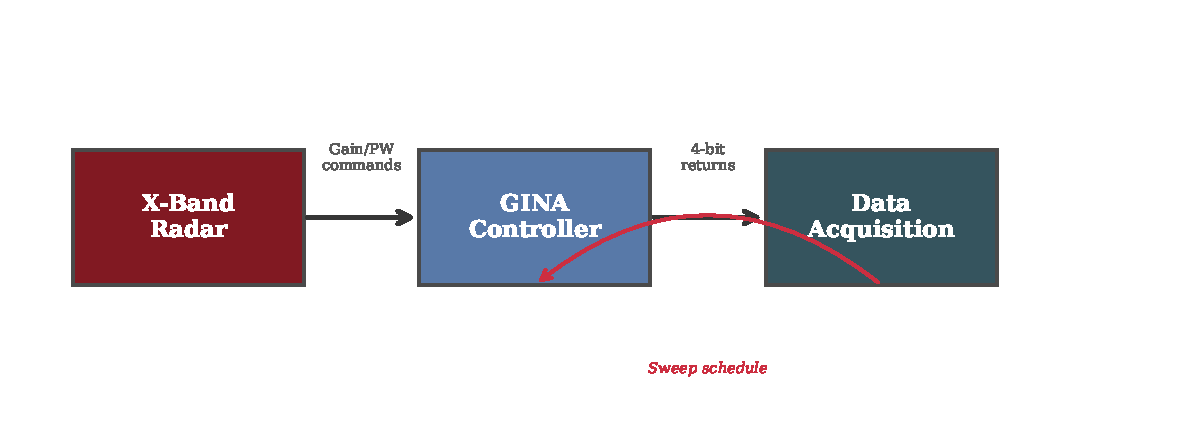
\includegraphics[width=\columnwidth]{figures/fig6_system_diagram.pdf}
\caption{System hardware configuration. The GINA controller issues gain and pulse width commands to the X-Band radar transceiver. Digitized 4-bit returns are logged by the data acquisition system, which also controls the sweep schedule. \textit{Placeholder---replace with actual hardware photo or detailed diagram.}}
\label{fig:system_diagram}
\end{figure}

\subsection{Radar Unit}
The radar used in this study is a Furuno DRS4D-NXT solid-state X-Band marine radar operating in the 9.38--9.44~GHz frequency band with a peak transmit power of 25~W. The unit employs a 24-inch (610~mm) radome-enclosed microstrip patch array antenna with a horizontal beamwidth of 3.9$^\circ$ and a vertical beamwidth of 25$^\circ$, providing an antenna gain of approximately 22--26~dBi. Returns are digitized at 4-bit resolution, producing 16 discrete amplitude levels per range cell. The total receiver dynamic range $G_{\text{total}}$ is not published by the manufacturer and is measured experimentally in this work (see Experiment~E2). The antenna assembly supports rotation speeds of 24, 36, and 48 revolutions per minute (RPM), with 48~RPM used as the default for gain-only sweeps and 24~RPM for combined gain and pulse width sweeps. The pulse repetition rate ranges from 700 to 1100~Hz depending on the selected range scale.

% TODO: Verify 4-bit ADC claim -- the DRS4D-NXT is a solid-state pulse
%       compression radar and may use a higher-resolution ADC internally.
%       Confirm what bit depth is presented at the data interface.

\subsection{Programmable Gain Controller}
Receiver gain is controlled through a programmable interface unit (GINA controller) connected between the radar transceiver and the data acquisition system, as shown in Fig.~\ref{fig:system_diagram}. The controller accepts serial commands that set the receiver gain to any integer value on a 0--100 scale. The dB-per-step calibration of this scale is measured experimentally (see Experiment~E2). Gain changes take effect within a single pulse repetition interval, enabling per-scan or per-sweep adjustment without interrupting antenna rotation.

% TODO: Add specifics on GINA controller communication protocol and latency.

\subsection{Data Acquisition}
Radar returns are captured as polar-coordinate images (range versus azimuth) at 4-bit depth for each antenna revolution. Each scan is timestamped and tagged with the gain and pulse width settings active during acquisition. Data is logged at the full rotation rate, yielding 48 scans per minute during gain-only sweeps and 24 scans per minute when pulse width variation is enabled.


% ====================================================================
% 3  METHODS
% ====================================================================
\section{Methods}

This section describes the three gain management strategies under comparison. All three operate on the same 4-bit intensity-only radar hardware described in the previous section and differ only in how receiver parameters are varied across successive scans.

\subsection{Method 1: Gain Sweep (HDR Reconstruction)}
The gain-sweep method ramps the receiver gain linearly from 0 to 100 across $N_g$ consecutive antenna revolutions. At each gain level $g_i$, a full 360$^\circ$ scan is recorded. Because the radar digitizes at 4-bit resolution, each scan captures only the targets whose return power falls within the 16-level window determined by the current gain.

At low gain settings, only the strongest reflectors (e.g., steel structures, large land masses) produce nonzero returns. As gain increases, progressively weaker targets appear, but strong reflectors saturate at the maximum digital count. By recording the gain level at which each target first appears (emerges from the noise floor) and the gain level at which it saturates, a reflectivity-versus-gain response curve is reconstructed for each resolution cell. This curve has far more than 4 bits of effective dynamic range, bounded by the number of gain steps and the stability of the scene. Figure~\ref{fig:waterfall} shows an example gain sweep waterfall, where the onset and saturation points of different targets are visible as distinct features along the gain axis.

\begin{figure}[t]
\centering
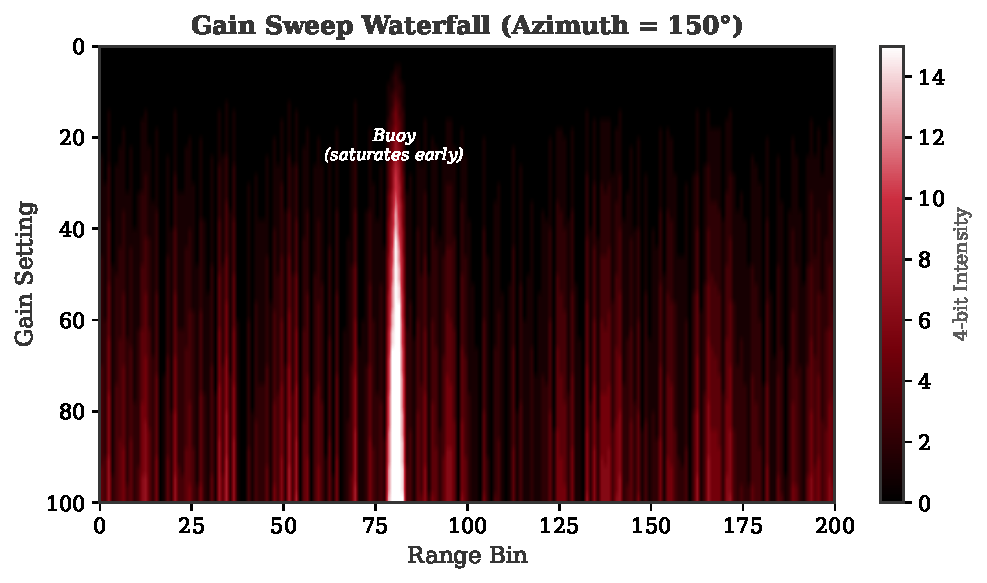
\includegraphics[width=\columnwidth]{figures/fig7_waterfall.pdf}
\caption{Gain sweep waterfall for a single azimuth slice. Each row represents one scan at a different gain setting. Strong reflectors appear at low gain and saturate early (left), while weaker targets emerge only at higher gain settings (right). The onset and saturation gain values encode reflectivity information beyond the native 4-bit depth. \textit{Placeholder---replace with real data.}}
\label{fig:waterfall}
\end{figure}

This method operates at the full antenna rotation speed of 48~RPM, with one gain step per revolution. A complete sweep through all gain levels requires $N_g$ revolutions. Stationary targets accumulate coherent responses across the sweep. Moving targets shift position between gain steps, producing radial or azimuthal streaking in the composite image, as illustrated in Fig.~\ref{fig:streaking}.

\begin{figure}[t]
\centering
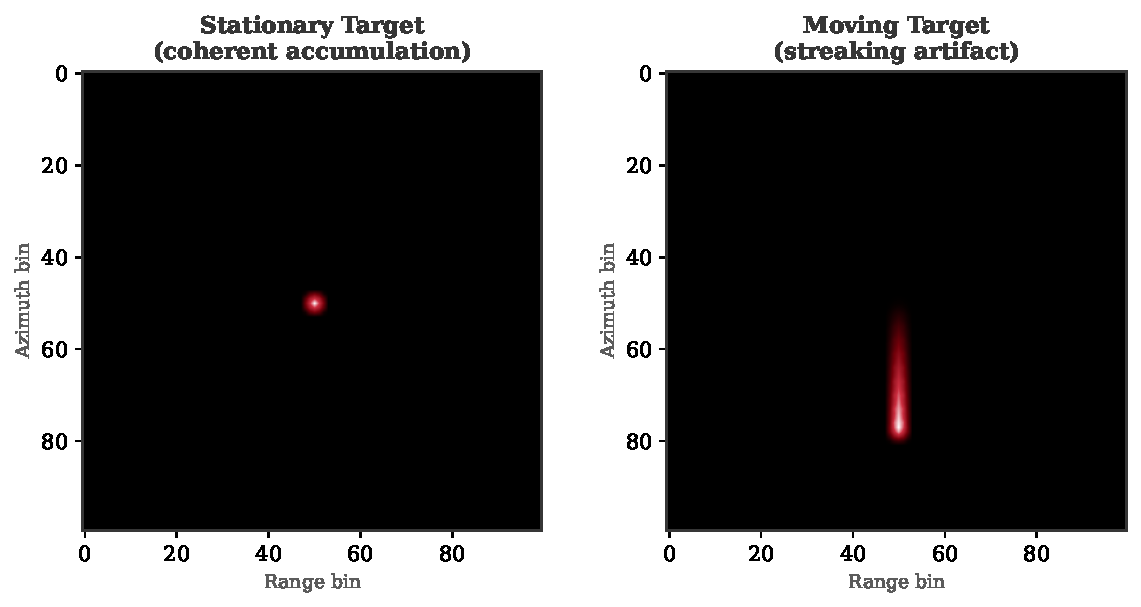
\includegraphics[width=\columnwidth]{figures/fig3_streaking.pdf}
\caption{Effect of target motion during a gain sweep. Left: a stationary target accumulates coherently across gain steps, producing a compact composite response. Right: a moving target shifts position between steps, producing a streaking artifact in the composite. \textit{Placeholder---replace with real data.}}
\label{fig:streaking}
\end{figure}

\subsection{Method 2: Gain and Pulse Width Sweep}
The second method extends the gain sweep by also varying the transmitted pulse width across a set of $N_p$ discrete values. Pulse width affects the energy on target and range resolution: longer pulses deposit more energy (improving detection of weak targets at the expense of range resolution), while shorter pulses preserve fine range discrimination~\cite{Richards2014Fundamentals}. Sweeping both parameters produces an $N_g \times N_p$ grid of acquisition configurations.

The additional pulse width variation introduces timing constraints that reduce the effective antenna rotation speed to 24~RPM. This lower rate doubles the time required per complete parameter sweep and increases exposure to motion artifacts. However, the two-dimensional parameter space captures information about target scattering behavior that gain variation alone cannot resolve, as the pulse width response encodes range-dependent characteristics independent of receiver amplification.

\subsection{Method 3: Temporal Filtering at Fixed High Gain}
The temporal filtering method operates at a fixed gain setting (high gain) and full rotation speed (48~RPM). Rather than sweeping parameters, it exploits the observation that radar returns from many targets exhibit natural intermittency. Targets whose returns fluctuate due to multipath effects, wave-induced obscuration, or marginal signal-to-noise ratios ``blink'' in and out across successive scans~\cite{Ward2013Marine}.

At fixed high gain, strong reflectors are saturated and merged in any single scan. However, by accumulating a temporal history of returns over $N_t$ consecutive scans, statistically distinct blinking patterns can reveal the presence of multiple targets within a merged region. A target that appears intermittently at a specific range--azimuth cell, while an adjacent merged target appears persistently, can be separated by its temporal signature. Figure~\ref{fig:temporal} illustrates this separation mechanism.

\begin{figure*}[t]
\centering
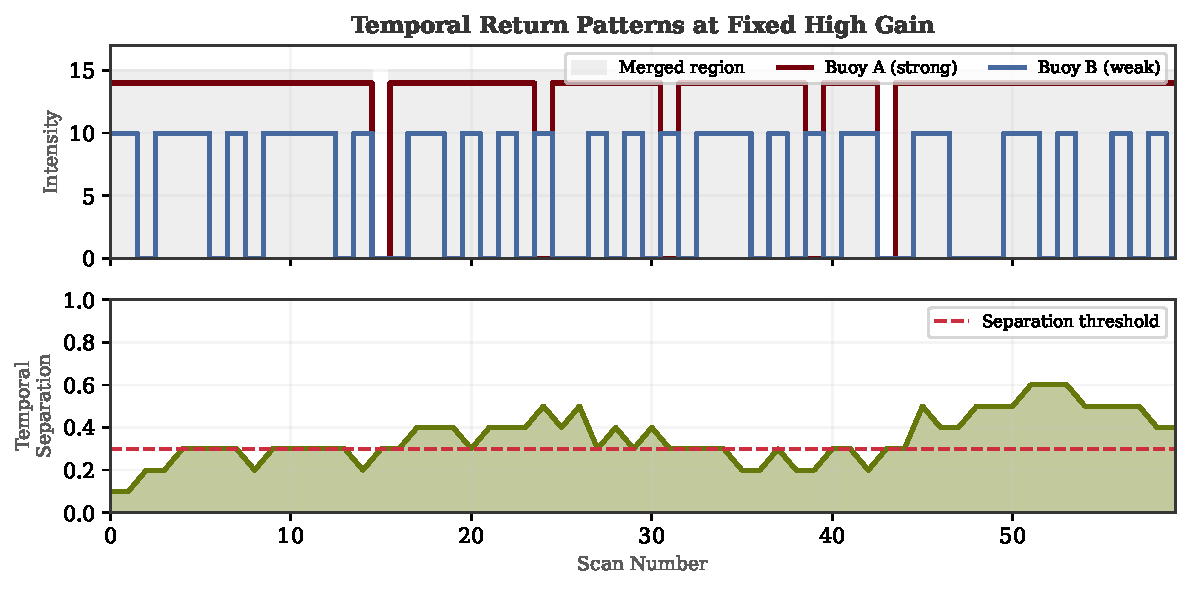
\includegraphics[width=\textwidth]{figures/fig4_temporal_filtering.pdf}
\caption{Temporal filtering for merged target separation. Top: return intensity over 60 consecutive scans at fixed high gain for two adjacent buoys. Buoy~A (strong) produces persistent returns, while Buoy~B (weak) blinks intermittently. Bottom: the rolling temporal separation metric distinguishes the two targets when it exceeds the threshold. \textit{Placeholder---replace with real data.}}
\label{fig:temporal}
\end{figure*}

This approach avoids the streaking artifacts inherent to parameter sweeping because all scans share the same receiver configuration. It is therefore compatible with dynamic scenes containing moving targets. The limitation is that it requires targets to exhibit sufficient temporal variability in their returns; two adjacent targets that both produce strong, persistent returns at high gain remain unresolvable.


% ====================================================================
% 4  EXPERIMENTAL SETUP
% ====================================================================
\section{Experimental Setup}

\subsection{Site and Targets}

% TODO: Fill in with actual experimental details.

Data was collected at [LOCATION] on [DATE] under [CONDITIONS: wind speed, wave height, visibility]. The scene contained metal navigation buoys at ranges of [X--Y]~m and shoreline features at ranges of [X--Y]~m. At least two buoys were positioned close enough in range--azimuth space that their returns merged at high gain settings, while a third buoy at greater range served as a weak target example.

% TODO: Add a figure showing the experimental geometry (overhead view of
%       radar location, buoy positions, and land features).

\subsection{Data Collection Runs}

Six data collection runs were performed at the same site during a single session. Table~\ref{tab:runs} summarizes the configuration and duration of each run.

\begin{table}[t]
\caption{Data collection schedule.}
\label{tab:runs}
\centering
\begin{tabular}{c l c c c}
\toprule
\textbf{Run} & \textbf{Description} & \textbf{RPM} & \textbf{Scans} & \textbf{Time} \\
\midrule
1a & Gain sweep (rep.\ 1) & 48 & 101 & $\sim$2 min \\
1b & Gain sweep (rep.\ 2) & 48 & 101 & $\sim$2 min \\
1c & Gain sweep (rep.\ 3) & 48 & 101 & $\sim$2 min \\
2a & Gain + PW sweep (rep.\ 1) & 24 & 606 & $\sim$25 min \\
2b & Gain + PW sweep (rep.\ 2) & 24 & 606 & $\sim$25 min \\
3\phantom{a} & Temporal baseline & 48 & 200 & $\sim$4 min \\
4\phantom{a} & Fixed low gain & 48 & 50 & $\sim$1 min \\
\bottomrule
\end{tabular}
\end{table}

Runs~1a--1c each ramp receiver gain linearly from 0 to 100 in unit increments ($N_g = 101$ steps), recording one full 360$^\circ$ scan per gain level at 48~RPM. Three repetitions are collected to assess repeatability.

Runs~2a--2b sweep gain from 0 to 100 for each of the six available pulse width settings (S1, S2, M1, M2, M3, L), yielding $101 \times 6 = 606$ scans per repetition at 24~RPM. Within each run, gain is swept completely for one pulse width before advancing to the next (i.e., G0--G100 at S1, then G0--G100 at S2, etc.), so that each pulse width sub-sweep is directly comparable to the gain-only data from Runs~1a--1c.

Run~3 operates at a fixed high gain setting and full rotation speed (48~RPM) for $N_t = 200$ consecutive scans ($\sim$4~min), providing the temporal observation window for intermittency-based target separation.

Run~4 operates at a fixed low gain setting for 50 scans, serving as a single-frame baseline for comparison.

\subsection{Experiments}

Table~\ref{tab:experiments} defines the six experiments performed on the collected data, each targeting a specific claim in this paper.

\begin{table*}[t]
\caption{Experiment definitions and corresponding data requirements.}
\label{tab:experiments}
\centering
\begin{tabular}{c l l l l}
\toprule
\textbf{Exp.} & \textbf{Name} & \textbf{Input Runs} & \textbf{Analysis} & \textbf{Output} \\
\midrule
E1 & Gain-response extraction & 1a--1c & Intensity vs.\ gain per target cell & Per-target gain-response curves \\
E2 & Radiometric resolution & 1a--1c & Onset/saturation gain, resolvable levels & Resolution improvement factor \\
E3 & Target merge/resolve & 1a--1c, 4 & Connected-component analysis vs.\ gain & Merge threshold per target pair \\
E4 & Temporal intermittency & 3 & Per-cell detection probability & Detection prob.\ histogram \\
E5 & Pulse width comparison & 2a--2b & Gain-response curves per PW & PW-dependent curve families \\
E6 & Sweep repeatability & 1a--1c & Cross-sweep standard deviation & Repeatability envelope \\
\bottomrule
\end{tabular}
\end{table*}

\textit{Experiment~E1: Gain-Response Extraction.} For each known target (buoys, land features), the range--azimuth cell(s) containing the target are identified across all 101 scans in a gain sweep. The digitized intensity at each gain level is recorded, producing a gain-response curve that characterizes how the target's apparent intensity evolves from noise floor emergence through saturation.

\textit{Experiment~E2: Radiometric Resolution.} The radiometric resolution improvement is quantified without assuming a specific ADC transfer function (linear, logarithmic, or otherwise). For each target, the \textit{onset gain} $g_{\text{onset}}$ (first gain at which intensity exceeds zero) and the \textit{saturation gain} $g_{\text{sat}}$ (first gain at which intensity reaches 15) are recorded. The \textit{onset-to-saturation span} $S = g_{\text{sat}} - g_{\text{onset}}$ characterizes the target's reflectivity footprint on the gain axis. The number of \textit{resolvable intensity levels} $L$ is then counted as the number of distinct intensity values observed across the span. A single fixed-gain frame provides at most 16 levels. The gain sweep provides up to $L$ levels per target, and targets can further be discriminated by their onset gain, saturation gain, and span values.

\textit{Experiment~E3: Target Merge/Resolve Analysis.} For each gain level in Runs~1a--1c, a thresholding and connected-component analysis determines whether two adjacent targets appear as one merged blob or two distinct returns. The merge threshold gain $g_{\text{merge}}$ is defined as the lowest gain at which the targets' connected components first overlap. The HDR composite is then evaluated to confirm that both targets are resolvable when the full gain sweep is used.

\textit{Experiment~E4: Temporal Intermittency.} For each range--azimuth cell in the scene, the detection probability $P_d$ is computed as the fraction of 200 consecutive scans (Run~3) in which the cell's intensity exceeds a noise threshold. Targets with $P_d > 0.8$ are classified as persistent; those with $P_d < 0.8$ are classified as intermittent. Two adjacent targets with differing persistence classes can be separated temporally even if they are spatially merged.

\textit{Experiment~E5: Pulse Width Comparison.} Gain-response curves are extracted from Runs~2a--2b for each pulse width setting independently. The six resulting curve families (one per pulse width) are compared to assess whether pulse width variation provides additional discriminative information beyond gain sweeping alone.

\textit{Experiment~E6: Sweep Repeatability.} The three independent gain sweeps (Runs~1a--1c) are compared point-by-point. For each target at each gain level, the standard deviation across the three repetitions is computed. Low variance indicates that the gain-response curve is a stable, repeatable measurement of the target's physical reflectivity characteristics rather than an artifact of noise.


% ====================================================================
% 5  RESULTS
% ====================================================================
\section{Results}

% NOTE: All figures in this section show theoretical/expected results.
% Replace with measured data after collection.

\subsection{Gain-Response Curves (E1)}

Figure~\ref{fig:gain_curves} shows measured digitized intensity as a function of receiver gain for four target types, averaged across three independent gain sweeps and smoothed with a Savitzky--Golay filter (window~11, order~2). The strong buoy produces a steep gain-response curve, emerging from the noise floor near gain~3 and reaching a plateau around gain~14. The moderate buoy follows a similar sigmoid shape but with a rightward shift, requiring approximately 5 additional gain steps to reach the same intensity. The weak buoy requires gain settings above~17 before producing detectable returns. The land target, a diffuse shoreline feature, exhibits a more gradual response due to its extended scattering geometry, rising later than the strong buoy but plateauing at a lower intensity. None of the four targets reaches the 4-bit ceiling of~16, indicating that even the strongest buoy does not fully saturate the digitizer at any gain setting. At any single fixed gain, only a narrow slice of this information is available. The full gain sweep recovers the complete response curve, providing effective dynamic range proportional to the number of gain steps.

\begin{figure}[t]
\centering
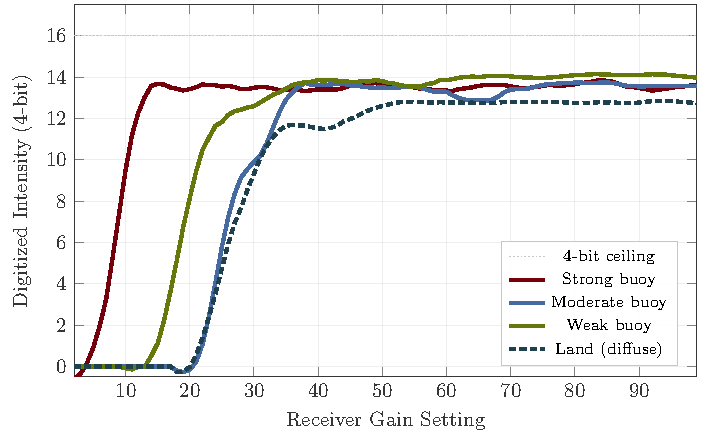
\includegraphics[width=\columnwidth]{figures/fig2_gain_response_curves.pdf}
\caption{Measured gain-response curves for four representative targets: a strong metal buoy, a moderate buoy, a weak buoy, and a diffuse land feature. Intensity is reported in 4-bit units (0--16). Each curve is the mean of three independent gain sweeps, smoothed with a Savitzky--Golay filter. The dashed line marks the 4-bit digitizer ceiling.}
\label{fig:gain_curves}
\end{figure}

\subsection{Radiometric Resolution (E2)}

The radiometric resolution improvement is characterized without assuming a specific relationship between the gain setting and physical signal power. Because the ADC transfer function (linear in amplitude, linear in power, logarithmic, or otherwise) is not published by the manufacturer, all results are reported in terms of directly observable quantities.

For each target, the onset gain $g_{\text{onset}}$ is the lowest gain at which the target produces a nonzero intensity, and the saturation gain $g_{\text{sat}}$ is the lowest gain at which the target reaches the 4-bit ceiling of 15. The onset-to-saturation span $S = g_{\text{sat}} - g_{\text{onset}}$ characterizes the target's footprint on the gain axis. A single fixed-gain frame provides at most 16 intensity levels per target. The gain sweep provides $L$ resolvable levels, where $L$ is the number of distinct intensity transitions observed across the span $S$. The \textit{resolution improvement factor} is defined as $R = L / 16$.

Figure~\ref{fig:dynamic_range_scaling} illustrates how the onset and saturation points differ across targets and how these measurements provide target discrimination without requiring knowledge of the ADC's dB-per-step calibration. Two targets with different spans $S$ or different onset gains $g_{\text{onset}}$ are distinguishable by their gain-response profiles even if they produce identical intensity values at any single fixed gain setting. This is the fundamental advantage of gain sweeping: it converts the gain axis into a discriminative feature that a single frame cannot provide.

\begin{figure}[t]
\centering
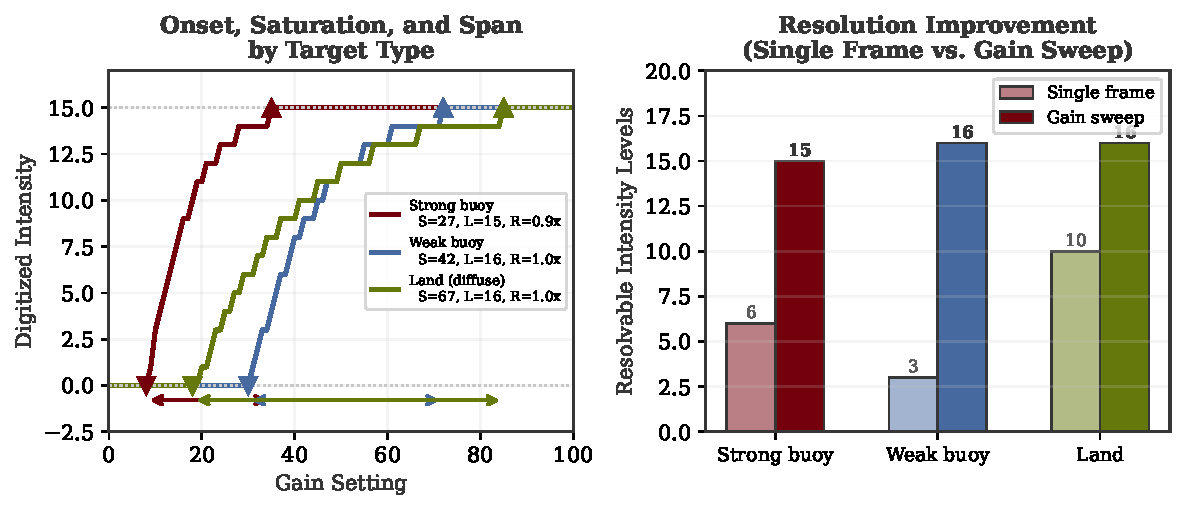
\includegraphics[width=\columnwidth]{figures/fig10_dynamic_range_scaling.pdf}
\caption{Expected onset and saturation points for targets of different reflectivity. The onset-to-saturation span $S$ and the resolution improvement factor $R = L/16$ quantify the gain sweep's benefit without assuming a dB calibration. \textit{Placeholder---replace with measured values.}}
\label{fig:dynamic_range_scaling}
\end{figure}

\subsection{Target Merge/Resolve Analysis (E3)}

The gain tradeoff illustrated in Fig.~\ref{fig:gain_tradeoff} is expected to manifest as a measurable merge threshold for each pair of adjacent targets. Figure~\ref{fig:merge_threshold} shows the expected behavior: as gain increases, each target's apparent spatial extent grows due to sidelobe amplification and saturation spreading, until the inter-target gap closes and the connected components merge. Below the merge threshold, both targets are individually resolved. Above it, they appear as a single blob. The HDR composite uses intensity information from below the merge threshold to recover individual target positions while retaining the weak-target sensitivity available only at higher gain.

\begin{figure}[t]
\centering
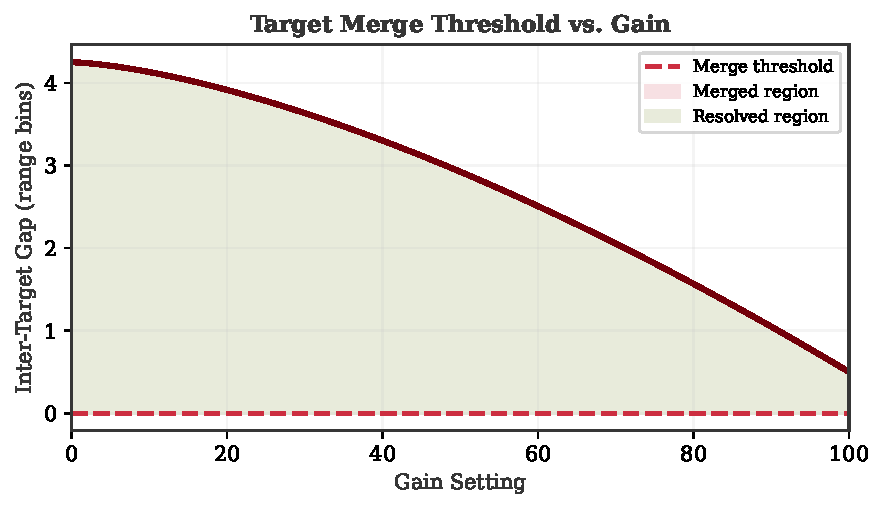
\includegraphics[width=\columnwidth]{figures/fig11_merge_threshold.pdf}
\caption{Expected inter-target gap as a function of gain. As gain increases, target returns expand spatially until the gap closes and targets merge. The HDR composite exploits the sub-threshold region where targets are individually resolved. \textit{Placeholder---replace with measured merge analysis.}}
\label{fig:merge_threshold}
\end{figure}

\subsection{Temporal Intermittency (E4)}

Figure~\ref{fig:detection_prob} shows the expected distribution of per-target detection probabilities at fixed high gain. Strong metal buoys and land features are expected to produce persistent returns ($P_d > 0.8$), while weaker or more distant buoys exhibit intermittent detection due to marginal signal-to-noise ratios and sea clutter fluctuations. Targets with sufficiently different $P_d$ values can be separated temporally even when they occupy overlapping spatial cells, as demonstrated by the temporal filtering mechanism in Fig.~\ref{fig:temporal}.

\begin{figure}[t]
\centering
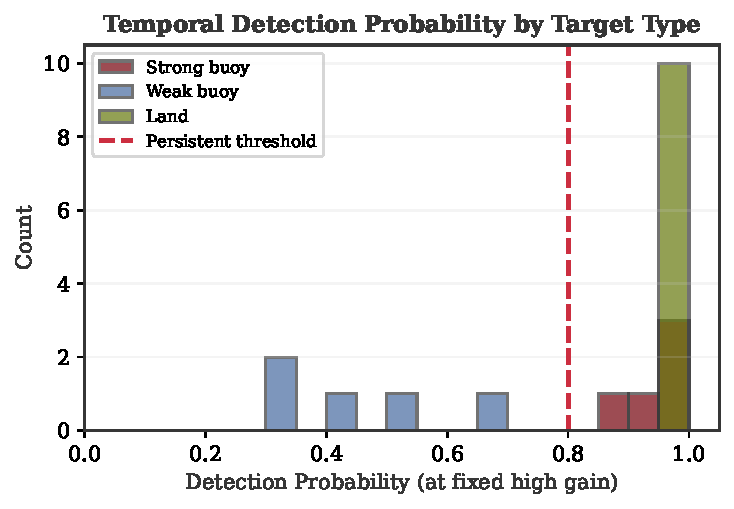
\includegraphics[width=\columnwidth]{figures/fig12_detection_probability.pdf}
\caption{Expected distribution of detection probabilities across target types at fixed high gain over 200 consecutive scans. Weak buoys exhibit lower, more variable detection rates, enabling temporal separation from persistent targets. \textit{Placeholder---replace with measured detection probabilities.}}
\label{fig:detection_prob}
\end{figure}

\subsection{Pulse Width Comparison (E5)}

Figure~\ref{fig:pw_comparison} shows the expected effect of pulse width on gain-response curves. Longer pulse widths (M3, L) deposit more energy on target, shifting the gain-response curve leftward (earlier onset, earlier saturation). Shorter pulse widths (S1, S2) require higher gain to achieve the same intensity but preserve finer range resolution. The separation between curves at different pulse widths carries information about target range extent and scattering geometry that gain variation alone does not capture.

\begin{figure*}[t]
\centering
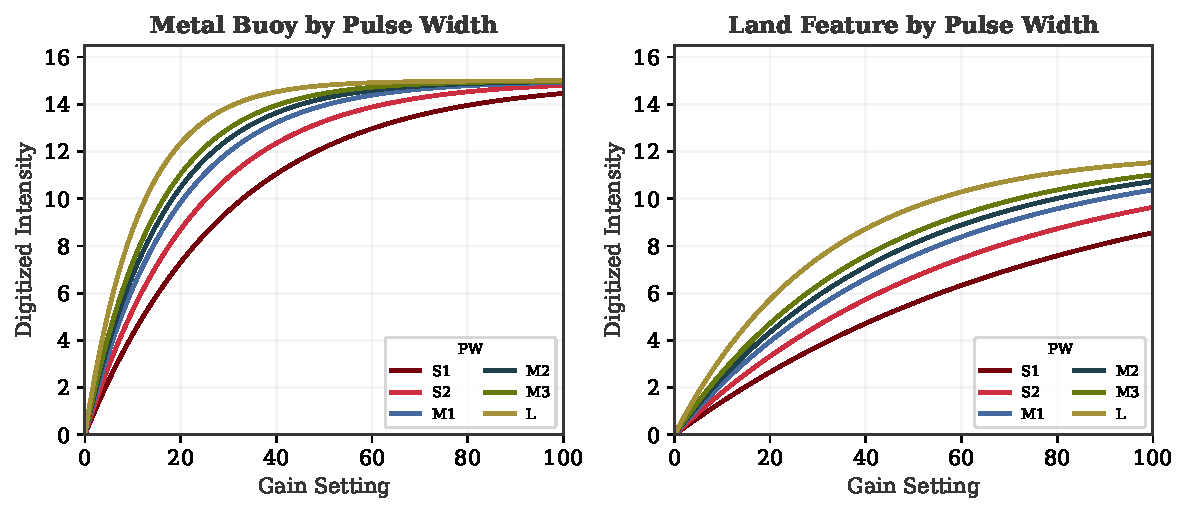
\includegraphics[width=\textwidth]{figures/fig9_pulse_width_comparison.pdf}
\caption{Expected gain-response curves at each of the six available pulse width settings. Left: metal buoy. Right: land feature. Longer pulses shift the response leftward due to increased energy on target. The inter-curve spacing encodes pulse-width-dependent scattering characteristics. \textit{Placeholder---replace with measured curves.}}
\label{fig:pw_comparison}
\end{figure*}

\subsection{Sweep Repeatability (E6)}

Figure~\ref{fig:repeatability} shows the expected repeatability of gain-response curves across three independent sweeps. For stationary targets, the three curves should closely overlap, with the $\pm 1\sigma$ envelope remaining narrow. Wider envelopes indicate gain levels where the target's return is near the noise floor or saturation boundary and therefore more sensitive to scan-to-scan fluctuations. Consistent overlap across repetitions validates that the gain-response curve reflects a stable physical property of the target rather than transient noise.

\begin{figure*}[t]
\centering
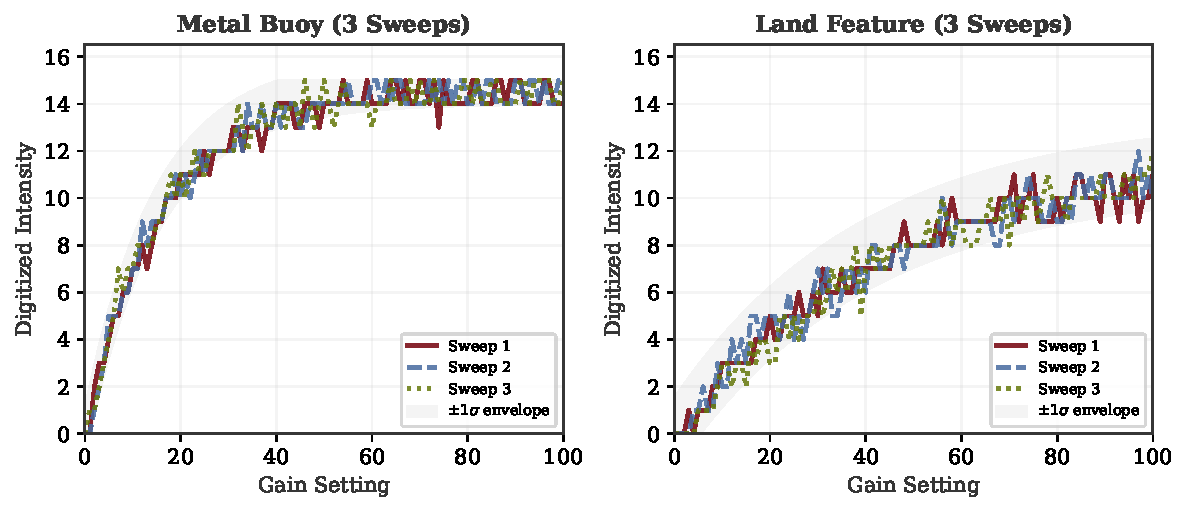
\includegraphics[width=\textwidth]{figures/fig8_repeatability.pdf}
\caption{Expected gain-response repeatability across three independent sweeps. Left: metal buoy. Right: land feature. The shaded envelope shows $\pm 1\sigma$ variation. Narrow envelopes indicate stable, reproducible measurements. \textit{Placeholder---replace with measured repeatability data.}}
\label{fig:repeatability}
\end{figure*}


% ====================================================================
% 6  DISCUSSION
% ====================================================================
\section{Discussion}

\begin{table}[t]
\caption{Comparison of gain management strategies.}
\label{tab:comparison}
\centering
\begin{tabular}{l c c c}
\toprule
 & \textbf{Gain} & \textbf{Gain +} & \textbf{Temporal} \\
 & \textbf{Sweep} & \textbf{Pulse Width} & \textbf{Filtering} \\
\midrule
Rotation speed (RPM) & 48 & 24 & 48 \\
Resolves merged targets & Yes & Yes & Yes \\
Detects weak targets & Yes & Yes & Yes \\
Resolvable intensity levels & $L$ (gain-dependent) & $L$ (gain + PW) & 16 (native) \\
Moving target handling & Streaking & Worse & No artifacts \\
Requires temporal variation & No & No & Yes \\
Parameter dimensions swept & 1 & 2 & 0 \\
\bottomrule
\end{tabular}
\end{table}

The three strategies, summarized in Table~\ref{tab:comparison} and Fig.~\ref{fig:method_comparison}, represent distinct points in a tradeoff space between dynamic range extension, temporal resolution, and scene compatibility.

\begin{figure*}[t]
\centering
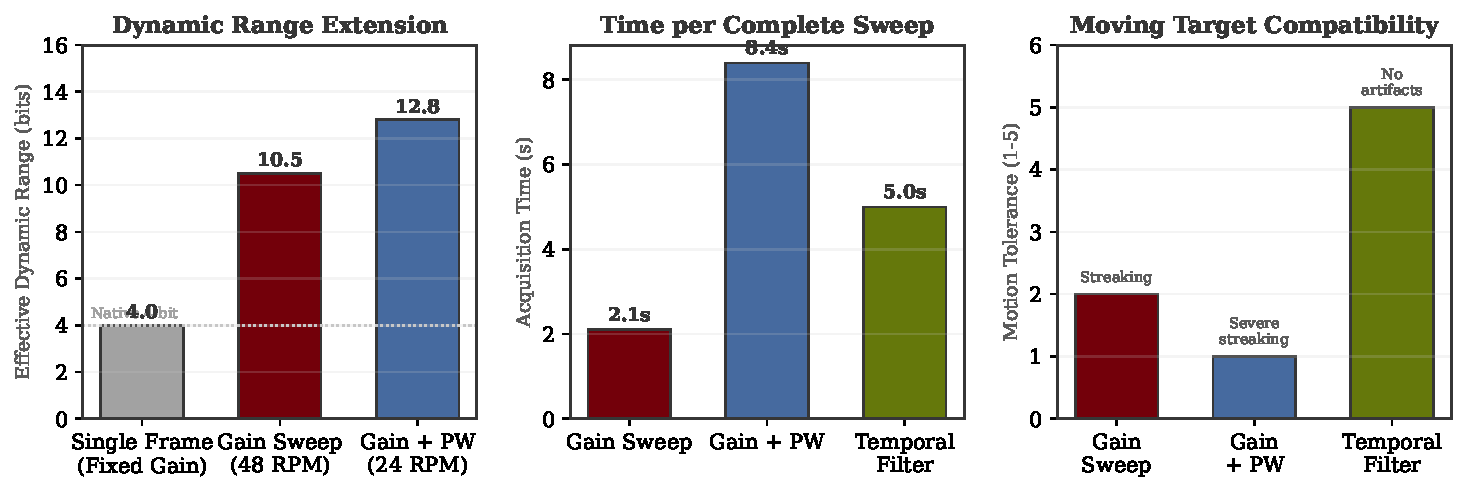
\includegraphics[width=\textwidth]{figures/fig5_method_comparison.pdf}
\caption{Quantitative comparison of the three gain management strategies. Left: effective dynamic range achieved beyond the native 4-bit resolution. Center: total acquisition time for a complete parameter sweep. Right: tolerance to moving targets on a qualitative scale. \textit{Placeholder---replace with measured values.}}
\label{fig:method_comparison}
\end{figure*}

The gain-sweep method provides the most general solution for stationary scene characterization. It operates at full rotation speed, requires no assumptions about target temporal behavior, and achieves a resolution improvement factor $R = L/16$ that scales with the number of gain steps in which a target produces distinct intensity transitions. Its primary limitation, motion-induced streaking, restricts its applicability to static or slowly changing environments such as infrastructure inspection and harbor mapping.

The gain-plus-pulse-width sweep offers a richer two-dimensional parameter space at the cost of halved rotation speed. The additional pulse width dimension captures range-dependent scattering characteristics that gain variation alone cannot resolve. However, the 24~RPM rotation rate doubles the time per sweep and worsens motion artifacts, making this method best suited for detailed characterization of known stationary targets where time is not constrained.

Temporal filtering at fixed high gain avoids parameter sweeping entirely and is therefore the only method compatible with fully dynamic scenes. It achieves target separation through a fundamentally different mechanism: statistical analysis of return intermittency rather than radiometric reconstruction. This approach requires no hardware modification beyond standard radar operation. Its limitation is the assumption that merged targets exhibit distinguishable temporal patterns. Two adjacent strong, persistent reflectors remain merged regardless of observation duration.

Machine learning approaches to radar target detection operate on single-frame or short-sequence data and have demonstrated strong performance on standard 4-bit imagery~\cite{Baird2020CNNLSTM, Wang2023SALALSTM, Chen2021PPInet}. These methods are complementary to, not competitive with, the approaches presented here. A neural network trained on 4-bit data can learn to detect and localize targets with high accuracy, but it cannot recover reflectivity information that the digitizer did not capture. The gain-sweep methods reconstruct radiometric data that no amount of post-processing can extract from a single fixed-gain scan, while ML methods provide detection capability that does not require parameter sweeping. A practical system may combine both: ML-based detection on standard scans for real-time situational awareness, with gain-swept characterization of regions of interest when detailed radiometric information is needed.


% ====================================================================
% 7  CONCLUSION
% ====================================================================
\section{Conclusion}

This paper compared three strategies for managing the sensitivity--resolution tradeoff inherent to low-bit-depth marine radar. Gain sweeping at full rotation speed (48~RPM) reconstructs extended reflectivity profiles of stationary targets, achieving radiometric resolution improvement factors well beyond the native 16 intensity levels of the 4-bit digitizer. Combined gain and pulse width sweeping provides richer target characterization at the cost of halved rotation rate (24~RPM) and increased motion sensitivity. Temporal filtering at fixed high gain separates merged targets through return intermittency analysis, maintaining compatibility with dynamic scenes but requiring targets with distinct temporal signatures.

Each method occupies a different region of the tradeoff space between radiometric fidelity, temporal resolution, and scene dynamics. The gain-sweep approach is recommended for infrastructure inspection and static scene mapping where maximum radiometric information is desired. Temporal filtering is preferred for navigational applications where moving targets are present and real-time operation is required. Combined gain and pulse width sweeping is appropriate for detailed offline characterization tasks where time constraints are relaxed.

These results demonstrate that programmable gain control enables commodity marine radar systems to exceed their native digitizer limitations through software-defined parameter management, providing enhanced sensing capability without hardware modification.


% ====================================================================
% REFERENCES
% ====================================================================
\bibliographystyle{asmeconf}
\bibliography{references}
\nocite{*}

\end{document}
